 \documentclass[a4paper,10pt]{article}
\input{/Users/WannaGetHigh/workspace/latex/macros.tex}

\title{VisA : TP Fuzzy C-Means}
\author{Fran\c cois \bsc{Lepan}}

\begin{document}
\maketitle

\section*{Introduction}

Dans ce TP nous allons voir comment segmenter une image couleur via la m\'ethode Fuzzy C-Means non supervis\'e.

\section{M\'ethode}

\begin{paragraph}{Initialisation}~\\

Pour commencer cette m\'ethode \`a besoin du nombre de cluster (classe). Avec ce nombre on initialise les centro\?ides al\'eatoirement  (non supervis\'e) ou en les s\'electionnant manuellement (supervis\'e). 

On stock chaque pixel dans une matrice $3*nombreDePixel$ : 3 pour l'espace RGB.

Ensuite on initialise une matrice de distance entre les pixels et les centro\?ides. Gr�ce \`a cette matrice on va en d\'eduire le degr\'e d'appartenance (comprit entre 0 et 1) des pixels par rapport a tous les cluster.
\end{paragraph}

\begin{paragraph}{Boucle principale}~\\

On va r\'ep\'eter n fois ces op\'eration, n \'etant demander \`a la base.

\begin{itemize}
\item on recalcule tout d'abord la position des centres des clusters d'apr\`es les distances et les degr\'es d'appartenance calcul\'es lors du tour pr\'ec\'edent.
\item on recalcule la distance de chaque pixel \`a ces nouveaux centres ainsi que leur degr\'e d'appartenance \`a chaque cluster.
\item on calcule la performance de l'algo.
\end{itemize}

\end{paragraph}

\newpage

\section{R\'esultat}

On voit sur la ~Fig.~\ref{seg_non_sup} que la m\'ethode non supervis\'e peut donner de tr\`es bon r\'esultat (\'equivalent \`a une m\'ethode supervis\'e).

\begin{figure}[ht]
\begin{center}
	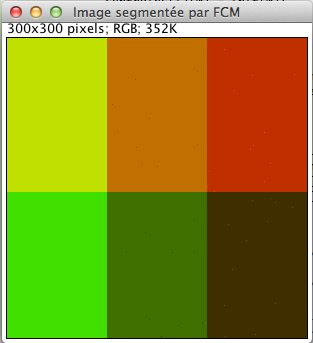
\includegraphics[width=4cm]{images/img_seg_non_sup}
	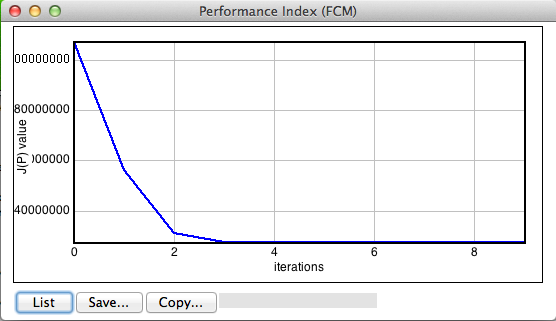
\includegraphics[width=7cm]{images/courbe_non_sup}
\end{center}
	\caption{A gauche l'image segment\'e et \`a droite la courbe de performance associ\'e.}
	\label{seg_non_sup}
\end{figure}

Mais elle peut aussi donner de mauvais r\'esultat (\emph{cf}.~Fig.~\ref{seg_non_sup_null}). Le probl\`eme viens du fait que deux centro\?ides se trouvent dans un m�me cluster.

\begin{figure}[ht]
\begin{center}
	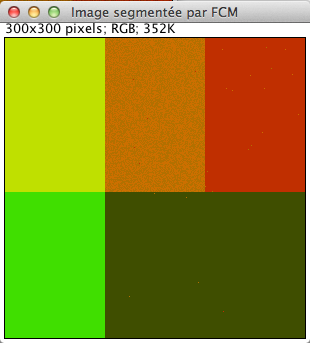
\includegraphics[width=4cm]{images/img_seg_non_sup_null}
	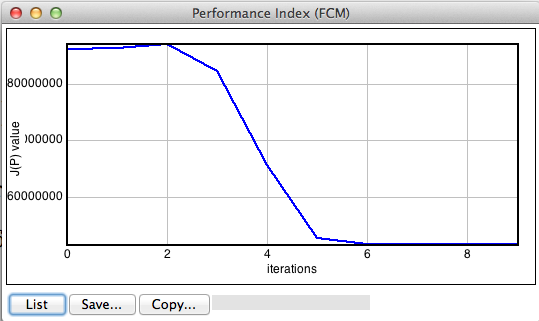
\includegraphics[width=7cm]{images/courbe_non_sup_null}
\end{center}
	\caption{A gauche l'image segment\'e et \`a droite la courbe de performance associ\'e.}
	\label{seg_non_sup_null}
\end{figure}



\section*{Conclusion}

Lors d'une utilisation supervis\'e cette m\'ethode segmente bien les images couleurs lorsque les centro\?ides sont bien plac\'e. Dans le cas contraire il se peux que deux centro\?ides soient \`a peut pr\`es au m�me endroit ne donnant pas des r\'esultats correcte. Une solution serait pour une m\'ethode non supervis\'e de contraindre les centro\?ides \`a ne pas �tre dans le m�me cluster.

\end{document}